% !TEX TS-program = pdflatex
% !TEX encoding = UTF-8 Unicode

% This is a simple template for a LaTeX document using the "article" class.
% See "book", "report", "letter" for other types of document.

\documentclass[11pt]{article} % use larger type; default would be 10pt

\usepackage[utf8]{inputenc} % set input encoding (not needed with XeLaTeX)

%%% Examples of Article customizations
% These packages are optional, depending whether you want the features they provide.
% See the LaTeX Companion or other references for full information.

%%% PAGE DIMENSIONS
\usepackage{geometry} % to change the page dimensions
\geometry{a4paper} % or letterpaper (US) or a5paper or....
% \geometry{margin=2in} % for example, change the margins to 2 inches all round
% \geometry{landscape} % set up the page for landscape
%   read geometry.pdf for detailed page layout information

\usepackage{graphicx} % support the \includegraphics command and options
\usepackage{alltt}
\usepackage{wrapfig}
% \usepackage[parfill]{parskip} % Activate to begin paragraphs with an empty line rather than an indent

%%% PACKAGES
\usepackage{booktabs} % for much better looking tables
\usepackage{array} % for better arrays (eg matrices) in maths
\usepackage{amssymb}
\usepackage{paralist} % very flexible & customisable lists (eg. enumerate/itemize, etc.)
\usepackage{verbatim} % adds environment for commenting out blocks of text & for better verbatim
\usepackage{subfig} % make it possible to include more than one captioned figure/table in a single float
% These packages are all incorporated in the memoir class to one degree or another...

%%% HEADERS & FOOTERS
\usepackage{fancyhdr} % This should be set AFTER setting up the page geometry
\pagestyle{fancy} % options: empty , plain , fancy
\renewcommand{\headrulewidth}{0pt} % customise the layout...
\lhead{}\chead{}\rhead{}
\lfoot{}\cfoot{\thepage}\rfoot{}

%%% SECTION TITLE APPEARANCE
\usepackage{sectsty}
\allsectionsfont{\sffamily\mdseries\upshape} % (See the fntguide.pdf for font help)
% (This matches ConTeXt defaults)

%%% ToC (table of contents) APPEARANCE
\usepackage[nottoc,notlof,notlot]{tocbibind} % Put the bibliography in the ToC
\usepackage[titles,subfigure]{tocloft} % Alter the style of the Table of Contents
\renewcommand{\cftsecfont}{\rmfamily\mdseries\upshape}
\renewcommand{\cftsecpagefont}{\rmfamily\mdseries\upshape} % No bold!

%%% END Article customizations

%%% The "real" document content comes below...

\title{Numerical Analysis Project 2}
\author{Margaret Dorsey}
%\date{} % Activate to display a given date or no date (if empty),
         % otherwise the current date is printed 

\newenvironment{claim}[1]{\par\noindent\underline{Claim:}\space#1}{}
\newenvironment{proof}[1]{\par\noindent\underline{Proof:}\space#1}{\hfill $\blacksquare$}

\begin{document}
\maketitle

\section*{Justification of Method}
	I elected to use cubic splines due to the discrete nature of the data set - because we have no guarantee of consistent, polynomial-like behavior at the data points, it is likely that a single interpolating polynomial would suffer from erratic behavior in between points to accommodate inconsistencies. Although Bezier Curves would likely provide a smooth, appealing interpolation of the data, because they do not necessarily agree with the data points, we would have less fine control over their behavior which is problematic for precise determination of ideal lighting. With  cubic splines, we can make adjustments solely through manipulation of the number, spacing, etc of data points without the need to also tweak control points to get expected behavior.
% will we need a root finding algorithm to recover the coefficients?
\par Additionally, to find $y$ values corresponding to a given $x$ value on a Bezier curve, we would need to find the roots of $x = (1-t)^3x_0 + 3(1-t)^2tx_1 + 3(1-t)t^2x_2$, giving us the $t$ corresponding to that $x$ value, and then use that to calculate $y(t)$. Although Newton's method is fast and reliable for cubic equations, it is still preferable to not do more work.

\subsection*{Computation of Splines}
\subsubsection*{Raw Output for Data Set 1}
\begin{alltt}
Coefficients for Data Set 1

0.000000	0.892633	0.923469	1.172533	0.000000	

 Values of Cubic Interpolant for Data Set 1
(-0.952381, -0.404201)
(-0.857143, -0.487113)
(-0.761905, -0.567712)
(-0.666667, -0.644455)
(-0.571429, -0.715801)
(-0.476190, -0.780210)
(-0.380952, -0.836615)
(-0.285714, -0.884856)
(-0.190476, -0.924882)
(-0.095238, -0.956637)
(0.000000, -0.980070)
(0.095238, -0.995064)
(0.190476, -1.001251)
(0.285714, -0.998202)
(0.380952, -0.985485)
(0.476190, -0.962672)
(0.571429, -0.929503)
(0.666667, -0.887225)
(0.761905, -0.837856)
(0.857143, -0.783424)
(0.952381, -0.725952)
\end{alltt}


\subsubsection*{Raw Output for Data Set 2}
\begin{alltt}
Coefficients for Data Set 2

0.000000	8.444919	-11.663674	8.724819	0.000000	

 Values of Cubic Interpolant for Data Set 2
(-0.952381, -0.433899)
(-0.857143, -0.569682)
(-0.761905, -0.683580)
(-0.666667, -0.761003)
(-0.571429, -0.787360)
(-0.476190, -0.748191)
(-0.380952, -0.644578)
(-0.285714, -0.507793)
(-0.190476, -0.372577)
(-0.095238, -0.273673)
(0.000000, -0.245820)
(0.095238, -0.312099)
(0.190476, -0.448947)
(0.285714, -0.621138)
(0.380952, -0.793448)
(0.476190, -0.930652)
(0.571429, -1.001062)
(0.666667, -1.003772)
(0.761905, -0.953724)
(0.857143, -0.865992)
(0.952381, -0.755650)
\end{alltt}
\subsection*{Plots of Output}
\subsubsection*{Data Set 1}
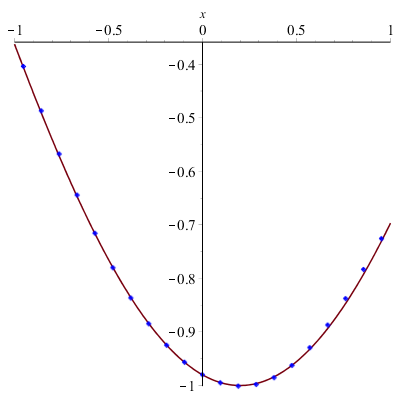
\includegraphics[scale=.5]{plots/dataset1approx.png}
\subsubsection*{Data Set 2}
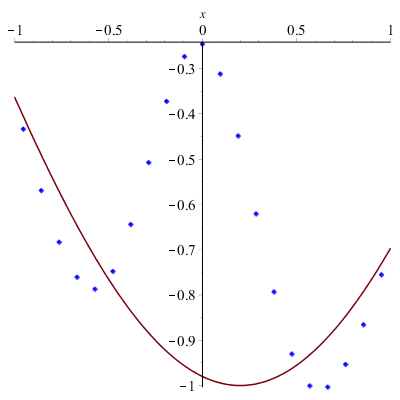
\includegraphics[scale=.5]{plots/dataset2approx.png}
\subsubsection*{Propagation of Error}
In order to maintain agreement in the first and second derivative, all of the data points changed, at least
slightly, when the center input point was changed signficantly (from $-.980070 $ to $-.245820$). However, the change in a 
given point becomes less and less the further away from the incorrect data the point is, so the error does not propagate
completely throughout, although it does effect the entire output set.

\subsection*{Testing and Maximum Error Bound}
\subsubsection*{$-\cos(x-.2)$}
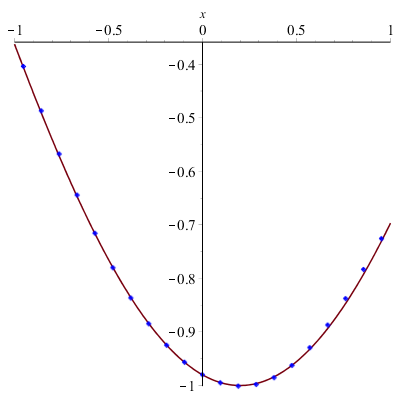
\includegraphics[scale=.3]{plots/dataset1approx.png}
$$
y(x) = \left\{
        \begin{array}{ll}
            -.94416178+0.01328678x+.297544285714286x^3+.892632857x^2 &  x < -.5 \\
            -.9800700-.20216250x+.4617342857x^2+0.01027857x^3 & x < 0 \\
 	-.98007000-.20216250x+.4617342857x^2+0.083021x^3 &  x < 0.5 \\
 	-.9208367857-.5575617857x+1.172532857x^2-.3908442857x^3 &  x \geq .5 \\
        \end{array}
    \right.
$$

The maximum error on the interval $[-1,1]$, $|-\cos(x-.2) - y(x)|$, is $0.00877438285370491$ at $x = .809398143755132$.
\subsubsection*{$1-x^2$}
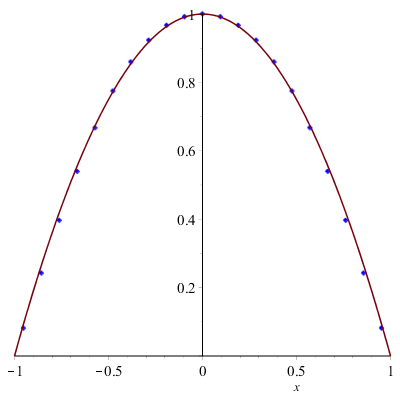
\includegraphics[scale=.3]{plots/dataset3approx.png}
$$
y(x) = \left\{
        \begin{array}{ll}
            -.8571428571x+.8571428571-.8571428571x^3-2.571428571x^2 &  x < -.5 \\
           1.00000000000000-.8571428571x^2+.28571428571x^3 & x < 0 \\
 	1.-.8571428571x^2-.28571428571x^3 &  x < 0.5 \\
 	.8571428571+.8571428571x-2.571428571x^2+.8571428571x^3 &  x \geq .5 \\
        \end{array}
    \right.
$$

The maximum error on the interval $[-1,1]$, $|1-x^2 - y(x)|$, is $0.0240658925870171$ at $x = -.811419518230411$.
\subsubsection*{$\sqrt{5-x^2}$}
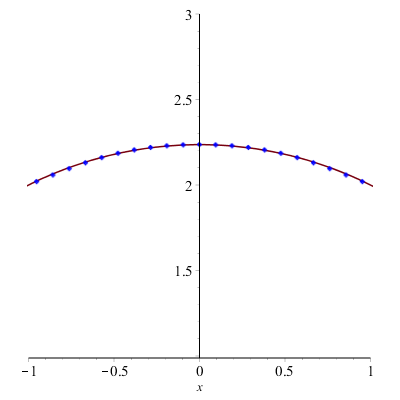
\includegraphics[scale=.3]{plots/dataset4approx.png}
$$
y(x) = \left\{
        \begin{array}{ll}
            2.1968628571-.2352308571x-.2160468571x^3-.648140571x^2 &  x < -.5 \\
           2.2360680-.1776788571x^2+0.09759428571x^3 & x < 0 \\
 	2.23606800+1.387778780781\times10^{-17}x-.1776788571x^2-0.09759428571*x^3 &  x < 0.5 \\
 	2.1968628571+.2352308571x-.648140571x^2+.2160468571 &  x \geq .5 \\
        \end{array}
    \right.
$$

The maximum error on the interval $[-1,1]$, $|-\sqrt{5-x^2} - y(x)|$, is $0.00723274707416888$ at $x = -.812835264258024$.

\subsubsection*{Conclusions}
\par In short, the program approximated all three functions fairly well, producing convincing graphs and relatively small maximum errors on the interval.

\newpage
\subsection*{Accuracy of Derivative Values}
\subsubsection*{$-\cos(x-.2)$}
\begin{alltt}
 Values of Cubic Interpolant for -cos(x-.2)

(-0.952381, -0.404201)
 dy/dx:	-0.877322

(-0.857143, -0.487113)
 dy/dx:	-0.861129

(-0.761905, -0.567712)
 dy/dx:	-0.828743

(-0.666667, -0.644455)
 dy/dx:	-0.780165

(-0.571429, -0.715801)
 dy/dx:	-0.715393

(-0.476190, -0.780210)
 dy/dx:	-0.634917

(-0.380952, -0.836615)
 dy/dx:	-0.549485

(-0.285714, -0.884856)
 dy/dx:	-0.463493

(-0.190476, -0.924882)
 dy/dx:	-0.376943

(-0.095238, -0.956637)
 dy/dx:	-0.289832

(0.000000, -0.980070)
 dy/dx:	-0.202162

(0.095238, -0.995064)
 dy/dx:	-0.111954

(0.190476, -1.001251)
 dy/dx:	-0.017227

(0.285714, -0.998202)
 dy/dx:	0.082017

(0.380952, -0.985485)
 dy/dx:	0.185780

(0.476190, -0.962672)
 dy/dx:	0.294062

(0.571429, -0.929503)
 dy/dx:	0.399608

(0.666667, -0.887225)
 dy/dx:	0.484690

(0.761905, -0.837856)
 dy/dx:	0.548501

(0.857143, -0.783424)
 dy/dx:	0.591042

(0.952381, -0.725952)
 dy/dx:	0.612312
\end{alltt}

\renewcommand{\arraystretch}{1.3} %<- modify cell height to give data breathing room
\begin{tabular}{| c | c c |}
\hline
$x$ & Spline Derivative & Actual Derivative \\
\hline
-0.952381 & -0.877322 &-.9137339606   \\
-0.857143 &-0.861129  & -.8709552164  \\
-0.761905 & -0.828743 & -.8202826368   \\
-0.666667 &-0.780165 & -.7621754887   \\
-0.571429 &  -0.715393& -.6971604219   \\
-0.476190 &	-0.634917 & -.6258259153   \\
-0.380952 &-0.549485  & -.5488200008   \\
-0.285714 &-0.463493 & -.4668398985   \\
-0.190476 &-0.376943 & -.3806286287 \\
-0.095238 &-0.289832 & -.2909675608   \\
0.000000 & -0.202162 & -.1986693308  \\
0.095238 & -0.111954  & -.1045704766 \\
0.190476 & -0.017227 &  -0.009523856019   \\
0.285714 & 0.082017& 0.08560908333   \\
0.380952 & 0.185780 & 0.1799661114   \\
0.476190 & 0.294062 & 0.2726920304   \\
0.571429 & 0.399608 & 0.3629473581   \\
0.666667 &  0.484690& 0.4499121782   \\
0.761905 & 	0.548501 & 0.5327992541  \\
0.857143 & 0.591042 &0.6108573450   \\
0.952381 &0.612312 & 0.6833789774   \\

\hline
\end{tabular} \\

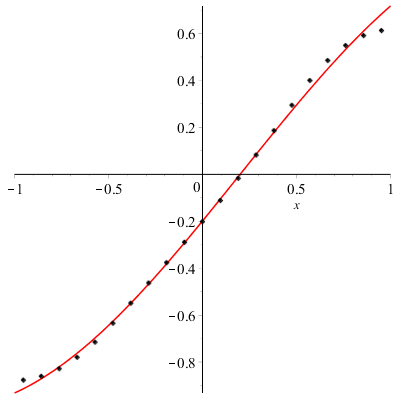
\includegraphics[scale=1]{plots/deriv1plot.png}
\newpage

\subsubsection*{$1-x^2$}
\begin{alltt}
 Values of Cubic Interpolant for 1-x^2
(-0.952381, 0.081540)
 dy/dx:	1.708455

(-0.857143, 0.242399)
 dy/dx:	1.661808

(-0.761905, 0.396594)
 dy/dx:	1.568513

(-0.666667, 0.539683)
 dy/dx:	1.428571

(-0.571429, 0.667222)
 dy/dx:	1.241983

(-0.476190, 0.774785)
 dy/dx:	1.010690

(-0.380952, 0.859812)
 dy/dx:	0.777454

(-0.285714, 0.923365)
 dy/dx:	0.559767

(-0.190476, 0.966927)
 dy/dx:	0.357629

(-0.095238, 0.991979)
 dy/dx:	0.171040

(0.000000, 1.000000)
 dy/dx:	0.000000

(0.095238, 0.991979)
 dy/dx:	-0.171040

(0.190476, 0.966927)
 dy/dx:	-0.357629

(0.285714, 0.923365)
 dy/dx:	-0.559767

(0.380952, 0.859812)
 dy/dx:	-0.777454

(0.476190, 0.774785)
 dy/dx:	-1.010690

(0.571429, 0.667222)
 dy/dx:	-1.241983

(0.666667, 0.539683)
 dy/dx:	-1.428571

(0.761905, 0.396594)
 dy/dx:	-1.568513

(0.857143, 0.242399)
 dy/dx:	-1.661808

(0.952381, 0.081540)
 dy/dx:	-1.708455

\end{alltt}

\begin{tabular}{| c | c c |}
\hline
$x$ & Spline Derivative & Actual Derivative\\
\hline
-0.952381 & 1.708455 &  1.904762 \\
-0.857143 & 1.661808 &  1.714286\\
-0.761905 & 1.568513 &   1.523810\\
-0.666667 & 1.428571 &  1.333334  \\
-0.571429 & 1.241983 &  1.142858 \\
-0.476190 & 1.010690 &  .952380 \\
-0.380952 &  0.777454&  .761904 \\
-0.285714 & 0.559767 &  .571428  \\
-0.190476 & 0.357629 &   .380952 \\
-0.095238 & 0.171040 &   0.190476\\
0.000000 &  0.000000&   0.000000 \\
0.095238 & -0.171040 & - 0.190476\\
0.190476 & -0.357629 &  -.380952 \\
0.285714 & -0.559767&  -.571428\\
0.380952 & -0.777454&  -.761904 \\
0.476190 & -1.010690 & -.952380  \\
0.571429 &-1.241983 &   -1.142858\\
0.666667 & -1.428571  &  -1.333334 \\
0.761905 &-1.568513 & -1.523810  \\
0.857143 & -1.661808 & -1.714286   \\
0.952381 &-1.708455 & -1.904762  \\

\hline
\end{tabular} \\
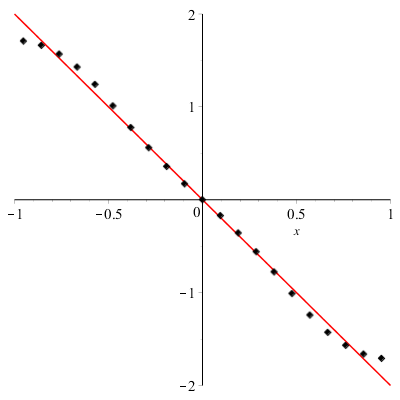
\includegraphics[scale=1]{plots/deriv2plot.png}
\newpage
\subsubsection*{$\sqrt{5-x^2}$}
\begin{alltt}
 Values of Cubic Interpolant for sqrt(5-x^2)
(-0.952381, 2.019639)
 dy/dx:	0.411442

(-0.857143, 2.058358)
 dy/dx:	0.399684

(-0.761905, 2.095396)
 dy/dx:	0.376168

(-0.666667, 2.129635)
 dy/dx:	0.340895

(-0.571429, 2.159955)
 dy/dx:	0.293864

(-0.476190, 2.185240)
 dy/dx:	0.235608

(-0.380952, 2.204887)
 dy/dx:	0.177863

(-0.285714, 2.219288)
 dy/dx:	0.125430

(-0.190476, 2.228947)
 dy/dx:	0.078308

(-0.095238, 2.234372)
 dy/dx:	0.036498

(0.000000, 2.236068)
 dy/dx:	0.000000

(0.095238, 2.234372)
 dy/dx:	-0.036498

(0.190476, 2.228947)
 dy/dx:	-0.078308

(0.285714, 2.219288)
 dy/dx:	-0.125430

(0.380952, 2.204887)
 dy/dx:	-0.177863

(0.476190, 2.185240)
 dy/dx:	-0.235608

(0.571429, 2.159955)
 dy/dx:	-0.293864

(0.666667, 2.129635)
 dy/dx:	-0.340895

(0.761905, 2.095396)
 dy/dx:	-0.376168

(0.857143, 2.058358)
 dy/dx:	-0.399684

(0.952381, 2.019639)
 dy/dx:	-0.411442

\end{alltt}

\begin{tabular}{| c | c c |}
\hline
$x$ & Spline Derivative & Actual Derivative\\
\hline
-0.952381 & 0.411442 &  0.4707511819  \\
-0.857143 & 0.399684 & 0.4150287594 \\
-0.761905 & 0.376168 &  0.3624217197  \\
-0.666667 & 0.340895  & 0.3123476952  \\
-0.571429 & 0.293864 & 0.2643276522  \\
-0.476190 & 0.235608 & 0.2179583417  \\
-0.380952 & 0.177863 & 0.1728945111  \\
-0.285714 & 0.125430 & 0.1288311943  \\
-0.190476 & 0.078308 & 0.08549420399  \\
-0.095238 & 0.036498 &  0.04263041293 \\
0.000000 & 0.000000 &  0.000000  \\
0.095238 & -0.036498 & -0.04263041293\\
0.190476 & -0.078308  &  -0.08549420399 \\
0.285714 &  -0.125430 & -.1288311943  \\
0.380952 & -0.177863  &  -.1728945111 \\
0.476190 & -0.235608 &  -.2179583417 \\
0.571429 &-0.293864  & -.2643276522  \\
0.666667 & -0.340895  &  -.3123476952 \\
0.761905 & -0.376168 &  -.3624217197  \\
0.857143 & -0.399684 &  -.4150287594 \\
0.952381 & -0.411442 &  -.4707511819 \\

\hline
\end{tabular} \\

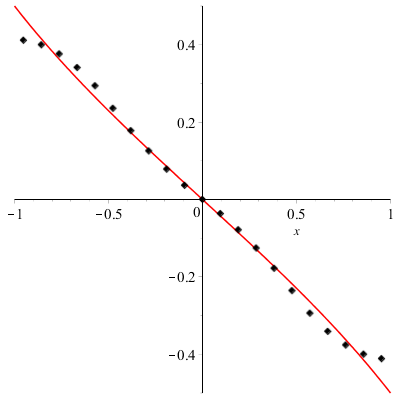
\includegraphics[scale=1]{plots/deriv3plot.png}
\subsubsection*{Analysis}
Without even calculating the error, it is clear from the plots that the derivative approximation is less accurate than
the approximation of the function itself. One cause of this is our natural endpoint condition - the first derivative of the spline
at the endpoints is affected by the second derivative going to $0$ - we could reduce this error by setting the second derivative
at the endpoints to the actual value of the second derivative.
\par The more pathological problem is that the derivative of an interpolating cubic is necessarily a quadratic - and parabolic approximations simply are not very flexible. Derivative functions that are well approximated by a parabola, like $-\sin$, have relatively little error in their approximation, while more error is induced by less suitable derivatives. This error is unavoidable when using cubic splines, and would have to be kept in mind when using them to approximate both the function and the first derivative.
\end{document}


 





